\documentclass{beamer}
\usepackage[utf8]{inputenc}
\usepackage{graphicx}

%%%%%%%%%%%%%%%%%%%%%%%%%%%%%%%%%%%%%%%%%%%%%%%%%%%%%%%%%%%%%%%%%%%%%%%%%%%%%%%

\title[Método de Newton]{Búsqueda de raíces mediante el método de Newton-Raphson}
\author[Técnicas Experimentales]{\textbf{Alba Crespo Pérez, Raquel Espino Mantas \\ y Robbert Jozef Michiels}}
\institute[ULL]{}
\date[12-05-2014]{12 de mayo de 2014}

%%%%%%%%%%%%%%%%%%%%%%%%%%%%%%%%%%%%%%%%%%%%%%%%%%%%%%%%%%%%%%%%%%%%%%%%%%%%%%%

\usetheme{Madrid}
\usecolortheme{beaver}

%%%%%%%%%%%%%%%%%%%%%%%%%%%%%%%%%%%%%%%%%%%%%%%%%%%%%%%%%%%%%%%%%%%%%%%%%%%%%%%

\begin{document}
  
%++++++++++++++++++++++++++++++++++++++++++++++++++++++++++++++++++++++++++++++

\begin{frame}

  \includegraphics[width=0.14\textwidth]{images/ull.eps}
  \hspace*{8cm}
  
\includegraphics[width=0.15\textwidth]{images/fmatesc.eps}
  \titlepage

  \begin{small}
    \begin{center}
     \emph{Facultad de Matemáticas} \\
     Universidad de La Laguna
    \end{center}
  \end{small}

\end{frame}

%++++++++++++++++++++++++++++++++++++++++++++++++++++++++++++++++++++++++++++++

%++++++++++++++++++++++++++++++++++++++++++++++++++++++++++++++++++++++++++++++

\begin{frame}
  \frametitle{Índice}
  \tableofcontents[pausesections]
\end{frame}

%++++++++++++++++++++++++++++++++++++++++++++++++++++++++++++++++++++++++++++++

\section{Motivación y objetivos}

%++++++++++++++++++++++++++++++++++++++++++++++++++++++++++++++++++++++++++++++

\begin{frame}

\frametitle{1. Motivación y objetivos}
\begin{block}{Objetivos generales y específicos} 

El \emph{objetivo principal} del presente trabajo reside en la implementación, mediante
el uso del lenguaje de programación Python, de un algoritmo basado en el método de 
Newton - Raphson que nos permita llevar a cabo el \textbf{cálculo de las raíces de la 
función} $\boldsymbol{f(x) = cos(\pi x)}$. \pause

Además, se pretende lograr la consecución de los siguientes \emph{objetivos específicos}:

    \begin{enumerate}
      \item
        Efectuar un \textbf{análisis numérico y gráfico} de la evolución en el \textbf{número 
        de iteraciones} requeridas por este método para la obtención de una raíz, \textbf{en 
        función del error absoluto} de la estimación inicial tomada como punto de partida del 
        método respecto a la solución real determinada tras su aplicación.
        \pause
      \item
         \textbf{Analizar el costo computacional}, en términos de tiempo de uso de CPU, 
         \textbf{asociado a la ejecución} del algoritmo implementado, así como su 
         sensibilidad ante modificaciones en los parámetros iniciales.
    \end{enumerate}

\end{block}
\end{frame}

%++++++++++++++++++++++++++++++++++++++++++++++++++++++++++++++++++++++++++++++

\section{Fundamentos teóricos}

%++++++++++++++++++++++++++++++++++++++++++++++++++++++++++++++++++++++++++++++

\subsection{Breve introducción histórica}
\begin{frame}
\frametitle{2.1. Breve introducción histórica}
\begin{block}{Origen del método y sus descubridores}

Este método constituye una \emph{vía algorítmica de análisis numérico} destinada a la 
\textbf{determinación de los ceros o raíces de una función} matemática.

    \begin{itemize} \pause
      \item
        Su primera descripción relevante fue realizada por \textbf{Isaac Newton} en su obra 
        \emph{De analysi per aequationes numero terminorum infinitas}, publicado en \textbf{1711}, 
        así como en su tratado \emph{De metodis fluxionum et serierum infinitarum}, editado en 
        1736 por John Colson bajo el título de \emph{Método de las fluxiones}.
        \pause
      \item 
        Sin embargo, si bien su reconocimiento no alcanzó en su momento la repercusión 
        otorgada a los trabajos de Newton, dicho método encuentra mención previa en el libro 
        \emph {Aequationum Universalis} (\textbf{1690}), cuya publicación conllevó para su autor, 
        el matemático inglés \textbf{Joseph Raphson}, la consecución del ingreso en la \emph{Royal 
        Society} de Londres.  
    \end{itemize}

\end{block}
\end{frame} 

%++++++++++++++++++++++++++++++++++++++++++++++++++++++++++++++++++++++++++++++

\subsection{Descripción teórica del método}
\begin{frame}
\frametitle{2.2. Descripción teórica del método}
\begin{block}{Análisis del procedimiento}
 
Para utilizar el método de Newton-Raphson es necesario comenzar con un \textbf{valor
inicial} suficientemente \textbf{cercano a la raíz buscada}, que a medida que avance 
la ejecución del algoritmo progresará acercándose al valor real de esta raíz. \pause 

Una vez fijada una estimación inicial $\boldsymbol{x_{0}}$, calcularemos la expresión 
de la \textbf{recta tangente} a la gráfica de la función \textbf{en el punto} $\boldsymbol
{x = x_{0}}$. La \textbf{coordenada de corte} de dicha recta \textbf{con el eje horizontal}
será considerada como un \textbf{valor más próximo} que $x_{0}$ a la raíz buscada, por lo 
que este paso podrá aplicarse de forma \emph{recursiva} tomando como suposición al nuevo 
valor obtenido hasta lograr una aproximación aceptable de la raíz, dentro de un \emph{margen 
de tolerancia} fijado de antemano. 

\end{block}
\end{frame}

%++++++++++++++++++++++++++++++++++++++++++++++++++++++++++++++++++++++++++++++

\begin{frame}
\frametitle{2.2. Descripción teórica del método}
\begin{block}{Obtención del algoritmo recursivo de Newton-Raphson}

Sabemos que la expresión de una recta de pendiente \emph{m} y que pasa por el punto $(a, b)$ 
viene por $ y - b = m (x - a)$. Por tanto, la expresión de la recta tangente a una función $f(x)$ 
en el punto $x = x_{0}$ queda como:
    \vspace*{-2mm}
    \begin{center}
    $\boldsymbol{y - f(x_{0}) = f'(x_{0}) (x - x_{0})}$
    \end{center}
    \vspace*{-2mm} \pause

Hallamos el punto de corte de la recta anterior con el eje de abscisas
\footnote{La notación $\boldsymbol{x_{n+1}}$ indica que el valor resultante de \emph{x} corresponderá 
a la estimación tomada como partida para la siguiente ejecución del algoritmo.}:
    \vspace*{-1mm}
    \begin{center}
    $y = 0 \ \ \to \ \ -f(x_{0}) = f'(x_{0}) (x_{n+1} - x_{0}) \ \ \to \ \ x_{0} f'(x_{0}) - f(x_{0}) 
    = x_{n+1} f'(x_{0}) \ \ \to \ \ \boldsymbol{x_{n+1} = x_{0} - \frac{f(x_{0})}{f'(x_{0})}}$
    \end{center}
    \vspace*{-1mm} \pause

Vemos así que las funciones con amplias variaciones de pendiente en el entorno de sus raíces 
dificultarán la convergencia del algoritmo, ante lo cual el establecimiento de una  \emph{cota 
máxima de iteraciones} nos permitirá detectar la aparición de patrones de divergencia.

\end{block}
\end{frame}

%++++++++++++++++++++++++++++++++++++++++++++++++++++++++++++++++++++++++++++++++++++++++++++++++

\subsection{Análisis de la función de estudio}
\begin{frame}
\frametitle{2.3. Análisis de la función de estudio}
\begin{block}{Cálculo teórico de raíces}

Con el objetivo de lograr una mejor comprensión de los resultados obtenidos en la aproximación de
las raíces de la función $f(x) = cos (\pi x)$ mediante el algoritmo de Newton-Raphson, procedemos 
a \textbf{calcular} dichas raíces \textbf{de modo teórico}, mediante la resolución de una sencilla 
\textbf{ecuación trigonométrica}: \pause
    \begin{center}
    $\boldsymbol{cos (\pi x) = 0} \ \ \to \ \ \pi x = \frac{\pi}{2} + k \pi, k \in \mathbb{Z} \ \ \to 
    \boldsymbol{x = \frac{1}{2} + k}, \ k \in \mathbb{Z}$
    \end{center}

\pause
Vemos así que se verifica lo siguiente:
    \begin{center}
    $cos (\pi x) = 0 \iff x = ..., -2.5, -1,5, -0.5, 0.5, 1.5, 2.5, ...$
    \end{center}

\pause
Concluimos de este modo que la función estudiada es \textbf{periódica}, con periodo \textbf{P = 2}. 

\end{block}
\end{frame}

%++++++++++++++++++++++++++++++++++++++++++++++++++++++++++++++++++++++++++++++++++++++++++++++++

\begin{frame}
\frametitle{2.3. Análisis de la función de estudio}
\begin{block}{Representación gráfica}

El carácter periódico de la función $\boldsymbol{f(x) = cos (\pi x)}$, así como el valor de sus 
raíces reales, quedan reflejados de modo ilustrativo a través de la siguiente gráfica: 

\vspace*{-3mm}

\begin{figure}[!th]
\begin{center}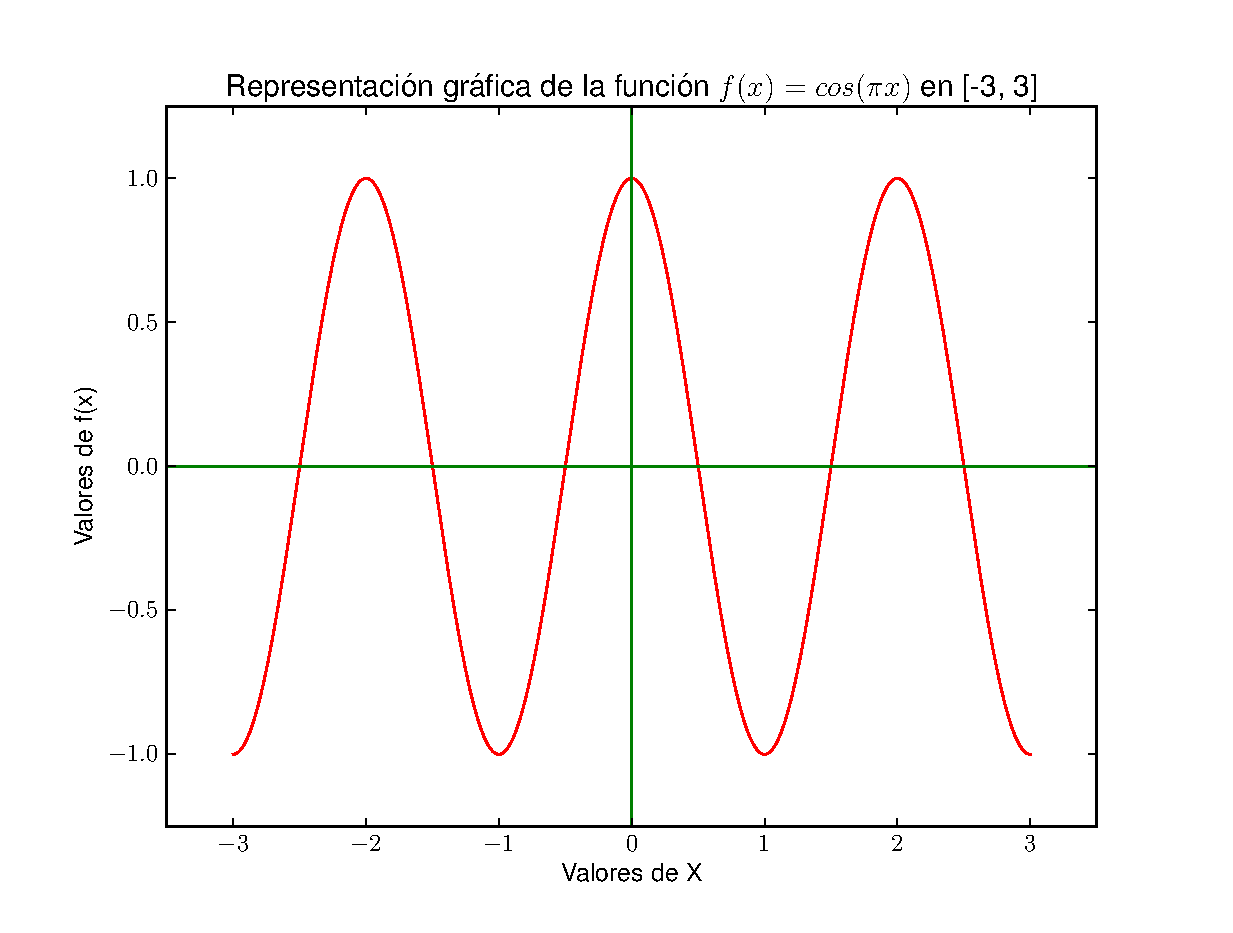
\includegraphics[height=5.5cm, width=8.5cm]{images/cos.eps}
\label{cos}
\end{center}
\end{figure}

\end{block}
\end{frame}

%++++++++++++++++++++++++++++++++++++++++++++++++++++++++++++++++++++++++++++++++++++++++++++++++

\begin{frame}
\frametitle{2.3. Análisis de la función de estudio}
\begin{block}{Puntos críticos y valores iniciales del algoritmo}

Debido a la naturaleza del método de Newton-Raphson, es preciso señalar que su aplicación no podrá
llevarse a cabo en caso de alcanzarse una \textbf{anulación de la derivada} para el punto de partida 
del algoritmo. \pause Analizaremos por tanto los \textbf{puntos críticos de la función} de estudio, 
para así conocer qué valores \textbf{deben ser evitados como suposiciones iniciales} a la hora de 
efectuar una invocación al método: \pause
    \begin{center}
    $\boldsymbol{(cos (\pi x))' = 0} \ \ \to \ \ -\pi sen (\pi x) = 0 \ \ \to \ \ sen (\pi x) = 0 \ \ \to$ 
    $\to\ \ \pi x = k \pi, \ k \in \mathbb{Z} \ \ \to \ \ \boldsymbol{x = k}, \ k \in \mathbb{Z} \ \ \to x = 
    ..., -2, -1, 1, 2, ...$
    \end{center}

\pause
Observamos así que los puntos críticos de la función $f(x) = cos (\pi x)$ se encuentran separados
una distancia de \emph{dos unidades}, lo que respalda las conclusiones obtenidas acerca de su 
periodicidad.

\end{block}
\end{frame}

%++++++++++++++++++++++++++++++++++++++++++++++++++++++++++++++++++++++++++++++

\section{Procedimiento experimental}

%++++++++++++++++++++++++++++++++++++++++++++++++++++++++++++++++++++++++++++++

\subsection{Descripción de los experimentos}
\begin{frame}
\frametitle{3.1. Descripción de los experimentos}
\begin{block}{Síntesis de los experimentos realizados}

    \begin{enumerate}
      \item
        Para llevar a cabo el cálculo de las raíces de la función objeto de estudio,
        se ha efectuado la \textbf{implementación de un algoritmo recursivo} basado 
        en el método \textbf{de Newton-Raphson}, en cuya ejecución hemos utilizado 
        \emph{distintos valores como parámetros iniciales} del método para así observar 
        los efectos producidos por la variabilidad de éstos sobre la solución final. 
        \pause
        \vspace*{-1mm}
      \item
        Ha sido diseñado un programa Python destinado a permitir el \textbf{recuento de 
        las iteraciones} requeridas para el cálculo de una raíz en función del error absoluto
        de la estimación inicial, \emph{almacenando los resultados en un fichero} para su 
        posterior lectura y \textbf{representación gráfica} por parte de un programa creado 
        a tal efecto.
        \pause
        \vspace*{-1mm}
      \item
        Con el fin de analizar el costo computacional del algoritmo, hemos realizado un
        diagrama que refleja el \textbf{tiempo total de CPU} empleado en distintas ejecuciones, 
        \textbf{frente al volumen de iteraciones} requerido durante las mismas.
    \end{enumerate}

\end{block}
\end{frame}

%++++++++++++++++++++++++++++++++++++++++++++++++++++++++++++++++++++++++++++++

\subsection{Descripción del material}
\begin{frame}
\frametitle{3.2. Descripción del material}
\begin{block}{Características de hardware y software}

Seguidamente se detallan las especificaciones técnicas de la computadora empleada
para llevar a cabo los experimentos, así como las versiones de los programas utlizados:
\pause

\begin{enumerate}

    \item
      \textbf{HARDWARE:}
      \begin{itemize}    
          \item
            \textbf{Tipo de CPU:} Pentium(R) Dual-Core CPU, GenuineIntel, T4500.
          \item
            \textbf{Velocidad de la CPU:} 1200 Hz.
          \item
            \textbf{Tamaño del caché:} 1024 KB.
          \item
            \textbf{Memoria RAM:} 8 GB.
      \end{itemize}

\pause

    \item
      \textbf{SOFTWARE:}
      \begin{itemize}
        \item      
          \textbf{Versión de Python:} 2.7.3.
        \item
          \textbf{Compilador Python:} GCC 4.7.2.
        \item
          \textbf{Sistema operativo:} Linux-3.5.0-17-genérico con Ubuntu-12.10-quantal.
        \item
          \textbf{Fecha de creación de la versión de Python:} Sep 26 2012 21:53:58.
      \end{itemize}

\end{enumerate}

\end{block}
\end{frame}

%++++++++++++++++++++++++++++++++++++++++++++++++++++++++++++++++++++++++++++++

\subsection{Resultados obtenidos}
\begin{frame}
\frametitle{3.3. Resultados obtenidos}
\begin{block}{Tabla ejemplificativa de raíces y parámetros de inicio}

\vspace*{-0.6cm}
\begin{table}
\end{table}
\begin{table}[H]
\begin{center}
\begin{tabular}{|c|c|c|c|c|}

   \hline
   \textbf{INICIO}  & \textbf{TOLERANCIA}  & \textbf{ITERACIONES } & \textbf{RESULTADO}  \\ \hline
   -7.08            & $10^{-7}$            & 3                     & -8.5                \\ \hline
   -7.1             & $10^{-7}$            & 4                     & -9.5                \\ \hline
   -7.2             & $10^{-7}$            & 3                     & -7.5                \\ \hline
   -5.8             & $10^{-5}$            & 2                     & -5.49999728877      \\ \hline
   -5.8             & $10^{-6}$            & 3                     & -5.5                \\ \hline
   -0.23            & $10^{-7}$            & 3                     & -0.5                \\ \hline
   -0.23            & $10^{-9}$            & 3                     & -0.5                \\ \hline
   1.24             & $10^{-6}$            & 2                     & 1.50000001507       \\ \hline
   1.24             & $10^{-8}$            & 3                     & 1.5                 \\ \hline
   2.17             & $10^{-12}$           & 4                     & 2.5                 \\ \hline
   3.45             & $10^{-4}$            & 1                     & 3.49999999976       \\ \hline
   3.45             & $10^{-10}$           & 2                     & 3.5                 \\ \hline

\end{tabular}
\end{center}
\label{nwtable}
\end{table}

\end{block}
\end{frame}

%++++++++++++++++++++++++++++++++++++++++++++++++++++++++++++++++++++++++++++++

\begin{frame}
\frametitle{3.3. Resultados obtenidos}
\begin{block}{Incremento en la cantidad de iteraciones frente a la variación de 
los errores absolutos iniciales}

\begin{figure}[!th]
\begin{center}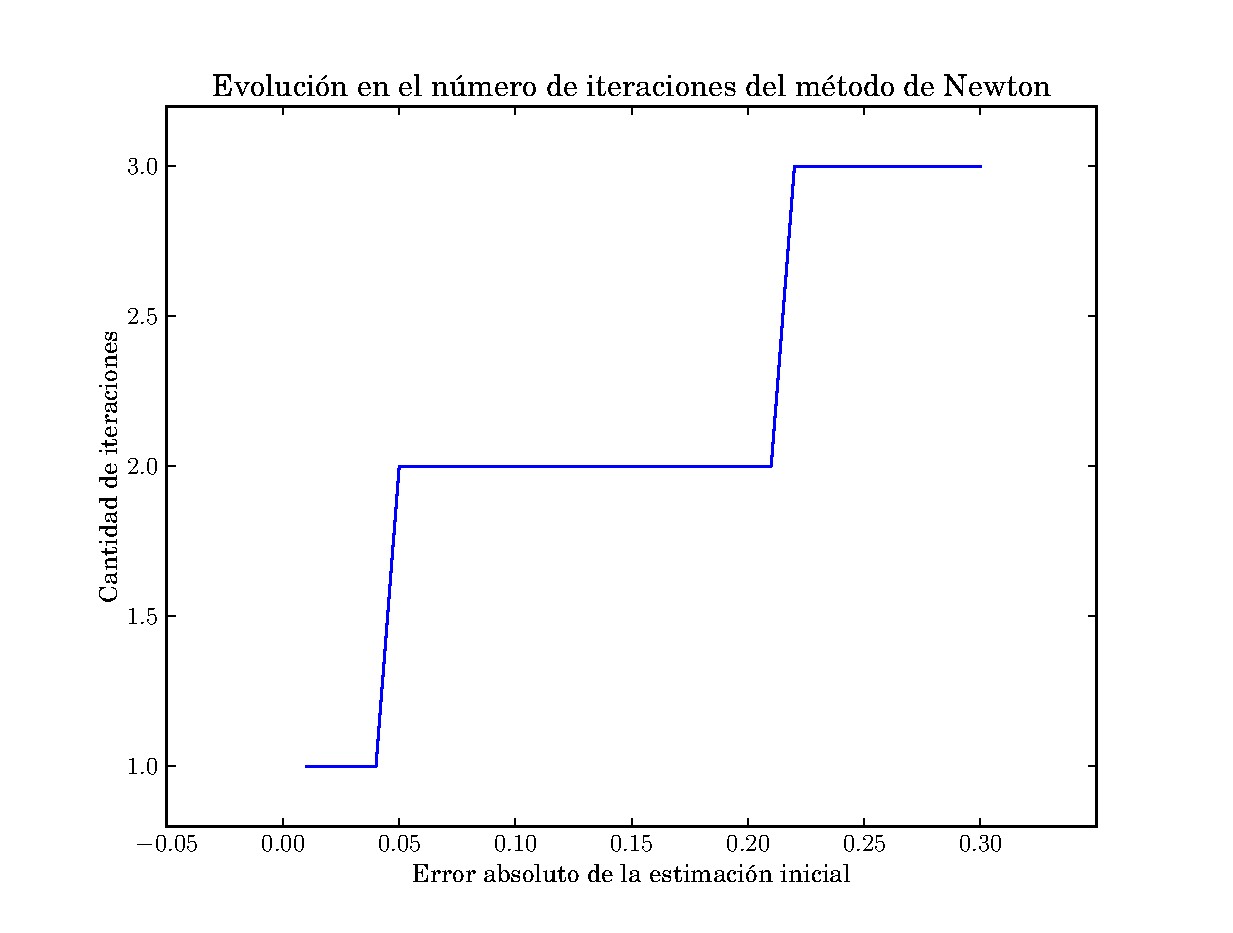
\includegraphics[height=6.5cm, width=8.5cm]{images/iterevol.eps}
\label{iter}
\end{center}
\end{figure}

\end{block}
\end{frame} 

%++++++++++++++++++++++++++++++++++++++++++++++++++++++++++++++++++++++++++++++

\begin{frame}
\frametitle{3.3. Resultados obtenidos}
\begin{block}{Tiempo total de uso de CPU por volumen de iteraciones}

\begin{figure}[!th]
\begin{center}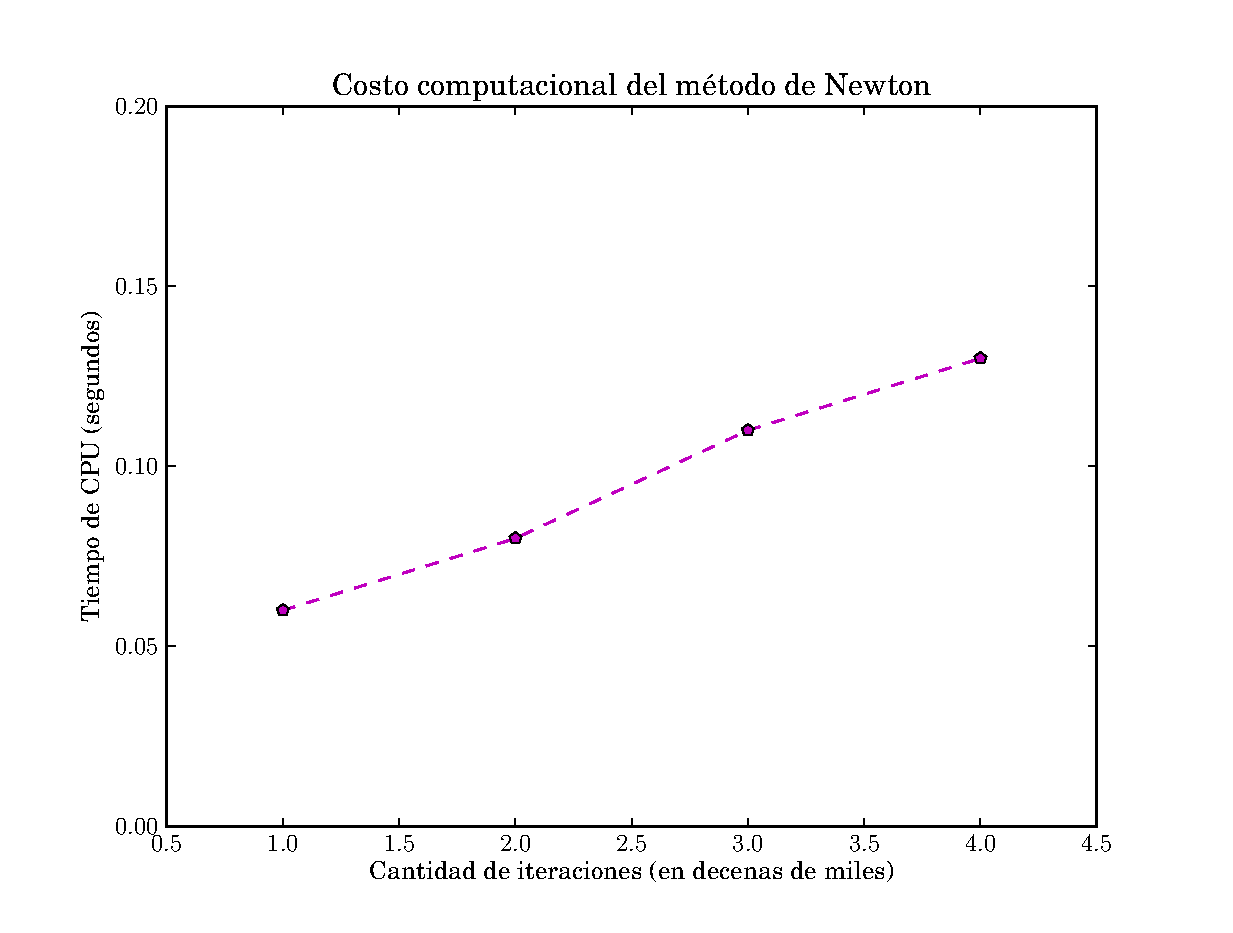
\includegraphics[height=6.5cm, width=8.5cm]{images/CPUtime.eps}
\label{iter}
\end{center}
\end{figure}

\end{block}
\end{frame} 

%++++++++++++++++++++++++++++++++++++++++++++++++++++++++++++++++++++++++++++++

\subsection{Análisis de los resultados}
\begin{frame}
\frametitle{3.4. Análisis de los resultados}
\begin{block}{Ejecución del algoritmo de Newton-Raphson}

\begin{itemize}
    \item
      En caso de proporcionar como suposición de partida un valor cercano a un \textbf
      {extremo relativo} de la función, \textbf{la iteración inicial} diverge respecto 
      a la raíz más próxima a dicho valor, puesto que la acentuada pendiente de la tangente 
      origina que su corte con la abscisa se encuentre notablemente alejado del valor de partida.
      \pause
      \vspace*{-0.1cm}
    \item
      \textbf{Todas las ejecuciones} que no comienzan con una anulación de la derivada \textbf
      {resultan convergentes}. Esto es así puesto que la periodicidad de la función permite que 
      los puntos originados en iteraciones divergentes propicien el inicio de una recursión 
      convergente.
      \pause
      \vspace*{-0.1cm}
    \item
      Observamos que el método de Newton-Raphson presenta una \textbf{elevada velocidad de 
      convergencia} para la función de estudio, puesto que la cantidad de iteraciones requerida 
      hasta lograr la obtención de una raíz válida no llega a superar las cuatro iteraciones, 
      aún en caso de seleccionar estrechos márgenes de tolerancia.  
\end{itemize}

\end{block}
\end{frame} 

%++++++++++++++++++++++++++++++++++++++++++++++++++++++++++++++++++++++++++++++

\begin{frame}
\frametitle{3.4. Análisis de los resultados}
\begin{block}{Evolución de las iteraciones y costo computacional}

\begin{itemize}
    \item
      Queda patente que el \textbf{incremento en el volumen de iteraciones} recursivas en 
      función del error absoluto de la estimación inicial muestra un \textbf{carácter suave}, 
      en conexión con la alta eficiencia y velocidad de convergencia del algoritmo.
      \pause
      \vspace*{-0.1cm}
    \item
      Sin embargo, la \textbf{separación constante} de una unidad existente \textbf{entre raíces 
      imposibilita el análisis} del comportamiento del método \textbf{para errores absolutos 
      superiores a 0.3} en la suposición de partida.
      \pause
      \vspace*{-0.1cm}
    \item
      La información relativa al costo computacional del algoritmo nos permite corroborar una vez 
      más la \textbf{notable eficiencia} del método, puesto que es preciso reiterar decenas de miles 
      de veces su invocación hasta obtener valores significativos para los tiempos de uso de CPU.
      \pause
      \vspace*{-0.1cm}
    \item
      Por último, observamos que \textbf{la variabilidad en los parámetros} iniciales \textbf{tan
      sólo afecta} a la utilización de recursos computacionales \textbf{cuando} su modificación 
      \textbf{altera el volumen de iteraciones requeridas} en la ejecución.
       
\end{itemize}

\end{block}
\end{frame}

%++++++++++++++++++++++++++++++++++++++++++++++++++++++++++++++++++++++++++++++

\section{Conclusiones}

%++++++++++++++++++++++++++++++++++++++++++++++++++++++++++++++++++++++++++++++

\begin{frame}
\frametitle{4. Conclusiones}
\begin{block}{Síntesis de conclusiones finales}

\begin{itemize}
    \item
      Las \textbf{raíces} de la función $f(x) = cos (\pi x)$ vienen dadas de la forma:
      \begin{center}
      $\boldsymbol{x = \frac{1}{2} + k}, \ k \in \mathbb{Z} \iff x = ..., -2.5, -1,5, -0.5, 0.5, 
      1.5, 2.5, ...$
      \end{center}
      \pause  
      \vspace*{-0.1cm}
    \item
      Para el caso de estudio, \textbf{la convergencia} del algoritmo de Newton-Raphson se encuentra 
      prácticamente \textbf{garantizada}, debido a la reducida separación entre raíces y a su carácter 
      de \textbf{periodicidad}.
      \pause  
      \vspace*{-0.1cm}
    \item
      La \textbf{eficiencia del algoritmo} implementado resulta considerablemente \textbf{elevada}, al 
      requerir ínfimos tiempos de CPU para la determinación de una raíz y no superar en ningún caso el 
      margen de cuatro iteraciones.
      \pause  
      \vspace*{-0.1cm}
    \item
      El método de Newton-Raphson demuestra caracterizarse por una \textbf{notable velocidad de 
      convergencia} para la función considerada, llegando a proporcionar hasta cinco cifras decimales 
      correctas a lo largo de una única iteración.
      \pause  
      \vspace*{-0.1cm}
    \item
      El reducido valor de los tiempos de CPU implica que las diferencias globales ante alteraciones
      en los parámetros iniciales pueden ser consideradas despreciables.
      
\end{itemize} 

\end{block}
\end{frame}

%++++++++++++++++++++++++++++++++++++++++++++++++++++++++++++++++++++++++++++++

\section{Bibliografía}

%++++++++++++++++++++++++++++++++++++++++++++++++++++++++++++++++++++++++++++++

\begin{frame}
  \frametitle{5. Bibliografía}

  \begin{thebibliography}{10}

    \beamertemplatebookbibitems
    \bibitem[1]{python}  
       \textsc{Alex Martelli}, \textit{Python: guía de referencia}, 
        Madrid, España, Anaya, 2003. 

    \beamertemplatebookbibitems
    \bibitem[2]{smk_metnum}  
       \textsc{A.A. Samarski}, \textit{Introducción a los métodos numéricos}, 
        Moscú, Rusia, MIR Editorial, 1986.

    \beamertemplatebookbibitems
    \bibitem[3]{chp_metnum}  
       \textsc{Steven C. Chapra}, \textit{Métodos numéricos para ingenieros}, 
        México, McGraw-Hill Interamericana de México, 2007.

    \beamertemplatebookbibitems
    \bibitem[4]{web_mwt} 
       Desarrollo histórico del método de Newton-Raphson y calculadora virtual de raíces:
       \begin{center}
       \scriptsize
          $http://www.uam.es/personal\_pdi/ciencias/barcelo/cnumerico/recursos/newton.html$
       \end{center}

  \end{thebibliography}
\end{frame}


%++++++++++++++++++++++++++++++++++++++++++++++++++++++++++++++++++++++++++++++

\end{document}

